\documentclass{article}

\usepackage{graphicx}
\usepackage{tikz}
\usepackage{tikzsymbols}
\usetikzlibrary{calc,patterns,shapes.geometric}
\pagestyle{empty}
\usepackage[margin=0pt]{geometry}
\geometry{papersize={14in,12in}}

\def\centerarc[#1](#2)(#3:#4:#5){\draw[#1] ($(#2)+({#5*cos(#3)},{#5*sin(#3)})$) arc (#3:#4:#5);}

\begin{document}
	\begin{figure}
		\centering
		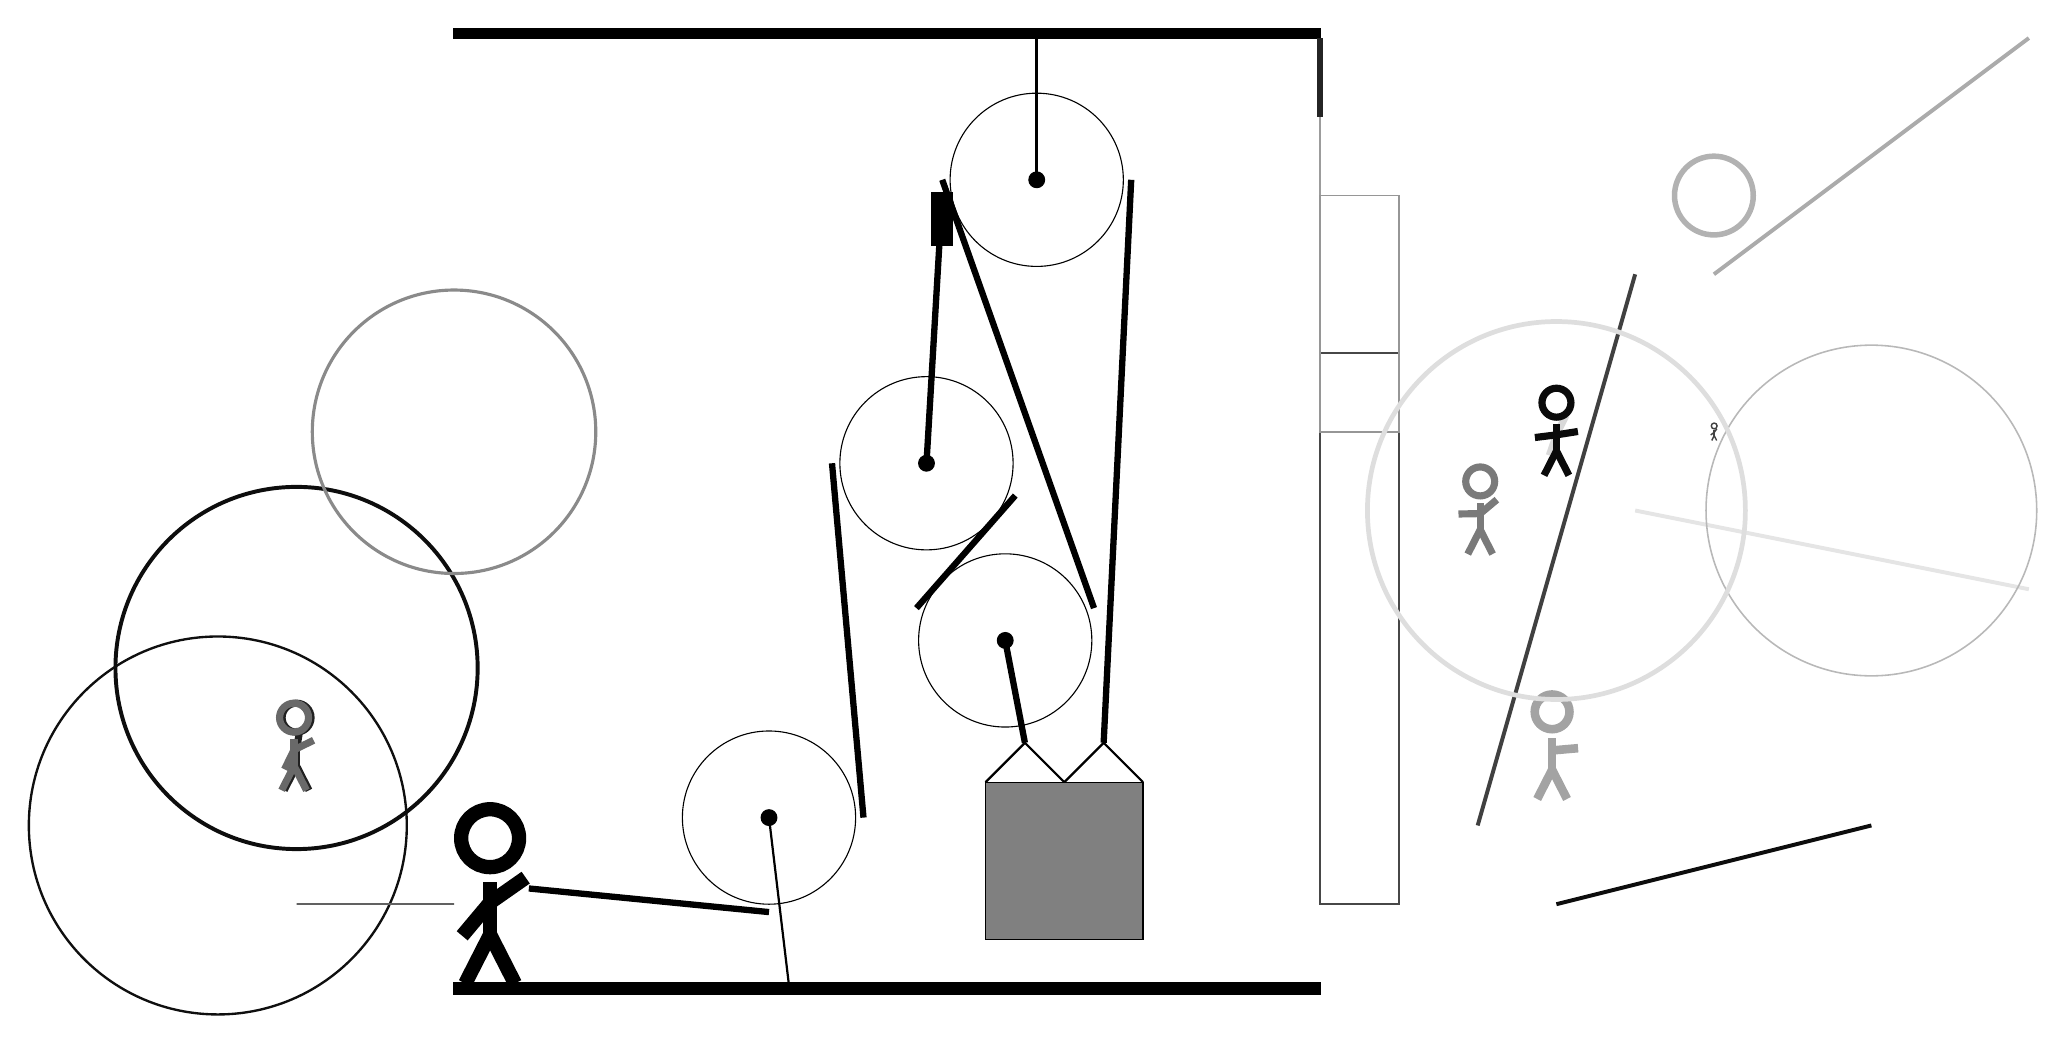
\begin{tikzpicture}
			%%%%% START %%%%%
			
			\draw[fill=black] (-6, 9) rectangle (5, 9.125);
			
			\draw (0, 3.6) circle (1.1);
			\draw[fill=black] (0, 3.6) circle (0.1);
			
			\draw (1, 1.35) circle (1.1);
			\draw[fill=black] (1, 1.35) circle (0.1);
			
			\draw (1.4, 7.2) circle (1.1);
			\draw[fill=black] (1.4, 7.2) circle (0.1);
			\draw[very thick] (1.4, 7.2) -- (1.4, 9);
			
			\draw [line width=0.3mm, color=black!94](-9, -1) circle (2.4);
			
			\draw[line width=0.5mm, color=black!33](10, 6) -- (14, 9);
			\node[line width=0.4mm, color=black!87] at (-8, 0) {\Strichmaxerl[5][72][81]};
			\node[line width=0.4mm, color=black!74] at (10, 4) {\Strichmaxerl[1][36][54]};
			
			\draw[line width=0.3mm, color=black!39] (5, 9) rectangle (5, 3);
			\draw[line width=0.5mm, color=black!10](9, 3) -- (14, 2);
			\draw[line width=0.5mm, color=black!95](8, -2) -- (12, -1);
			
			\node[line width=0.7mm, color=black!15] at (8, 4) {\Strichmaxerl[5][71][64]};
			\node[line width=0.7mm, color=black!96] at (8, 4) {\Strichmaxerl[5][7][9]};
			\draw[line width=0.3mm, color=black!72] (6, -2) rectangle (5, 5);
			\draw [line width=0.5mm, color=black!95](-8, 1) circle (2.3);
			
			\node[line width=0.5mm, color=black!36] at (8, 0) {\Strichmaxerl[6][90][5]};
			\draw[line width=0.2mm, color=black!62] (-8, -2) rectangle (-6, -2);
			
			\draw[line width=0.7mm, color=black!86] (5, 9) rectangle (5, 8);
			\draw [line width=0.7mm, color=black!30](10, 7) circle (0.5);
			\draw [line width=0.4mm, color=black!46](-6, 4) circle (1.8);
			
			\draw [line width=0.2mm, color=black!28](12, 3) circle (2.1);
			\draw[line width=0.5mm, color=black!75](7, -1) -- (9, 6);
			\node[line width=0.4mm, color=black!59] at (-8, 0) {\Strichmaxerl[5][64][26]};
			
			\draw[line width=0.2mm, color=black!41] (6, 4) rectangle (5, 7);
			\node[line width=0.3mm, color=black!52] at (7, 3) {\Strichmaxerl[5][1][40]};
			\draw [line width=0.6mm, color=black!13](8, 3) circle (2.4);
			
			\draw (-2, -0.9) circle (1.1);
			\draw[fill=black] (-2, -0.9) circle (0.1);
			\draw[thick] (-2, -0.9) -- (-1.75, -3);
			
			
			\draw[thick]  (0.75, -0.45) -- (1.25, 0.05) -- (1.75, -0.45) -- (2.25, 0.05) -- (2.75, -0.45);
			\draw[fill=black!50] (0.75, -0.45) rectangle (2.75, -2.45);
			\draw[line width=0.8mm] (-5.05, -1.8) -- (-2, -2.1);
			\centerarc[line width=0.8mm](-2, -0.9)(270:360:1.2000000000000002);
			\draw[line width=0.8mm] (-0.8, -0.9) -- (-1.2, 3.6);
			\draw[line width=0.8mm] (0, 3.6) -- (0.2, 7.0);
			\draw[line width=0.8mm, fill=black](0.1, 6.4) rectangle (0.3, 7.0);
			\centerarc[line width=0.8mm](0, 3.6)(-20:180:1.2000000000000002);
			\draw[line width=0.8mm] (1.1276, 3.1896) -- (-0.1276, 1.7604);
			\centerarc[line width=0.8mm](1, 1.35)(160:380:1.2000000000000002);
			\draw[line width=0.8mm] (2.1276, 1.7604) -- (0.2, 7.2);
			\draw[line width=0.8mm](1, 1.35) -- (1.25, 0.05);
			\centerarc[line width=0.8mm](1.4, 7.2)(0:180:1.2000000000000002);
			\draw[line width=0.8mm] (2.6, 7.2) -- (2.25, 0.05);
			
			\node at (-5.5, -1.9) {\Strichmaxerl[10][50][35]};
			
			\draw[fill=black] (-6, -3) rectangle (5, -3.15);
			
			%%%%% END %%%%%
		\end{tikzpicture}
	\end{figure}	
\end{document}